

\chapter{Sistema de controlo e monitorização: arquitetura e modelação}


Este capítulo tem como objetivo a descrição do sistema que resultou do trabalho prático
desta dissertação. Para esse fim, cada elemento pertencente ao sistema é caracterizado de
acordo com as suas funções, especificidades e respectiva arquitetura. É também descrito como os elementos interagem entre si. É também apresentado todo o processo de modelação do sistema tendo por base os requisitos adquiridos pelo cliente. 



%Dashboard - Interface que apresenta a informação mais importante para o utilizador de forma apelativa, tornando mais fácil a interacção e respetiva leitura


% Mockups - Design que a plataforma deverá apresentar no fim do seu desenvolvimento.



\section{Descrição global do sistema}

Este sistema tem como objetivo a supervisão remota da produção de salicornia,  permitindo não só a monitorização dos dados adquiridos pelos sensores, como também da atuação remota de determinados comandos. Neste contexto também será possível a aquisição de imagens que possibilitará a deteção de intrusos nas quintas onde se produz esta espécie.


\begin{figure}[!htb]
	\centering
	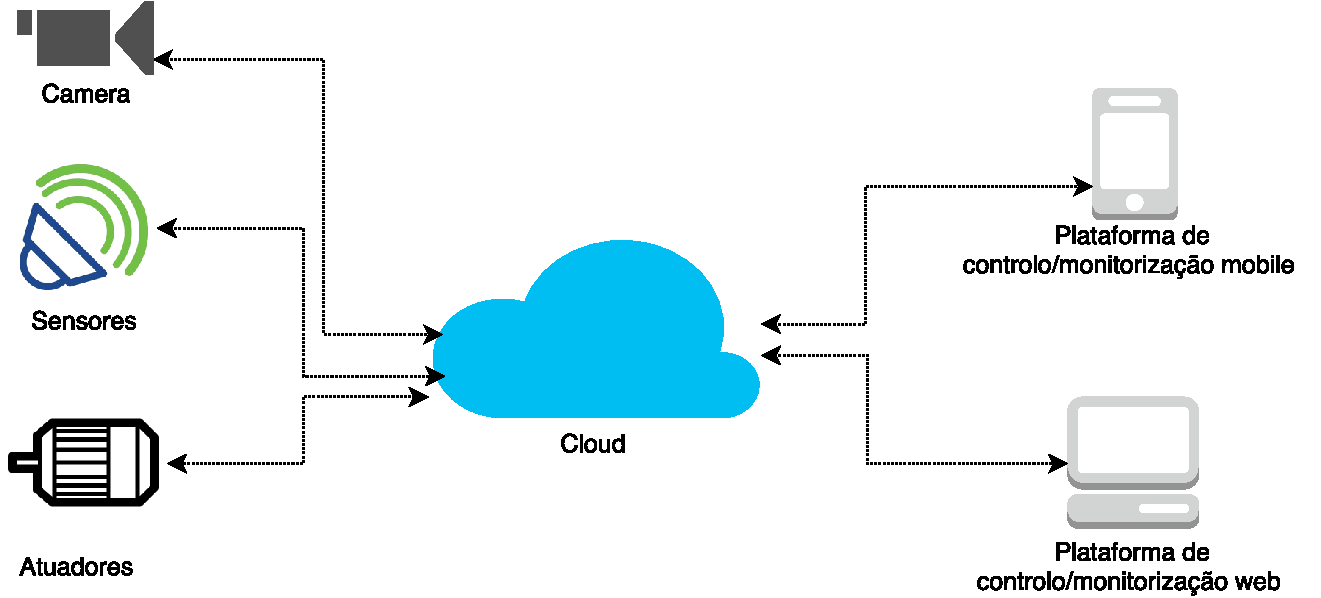
\includegraphics[scale=0.40]{esquemas/global_arquitetura.pdf}
	\caption{Ilustração principais componentes}
	\label{componentesall}
\end{figure}



O esquema da figura \ref{componentesall} ilustra todos os componentes de um modo geral e as diferentes plataformas com que o cliente pode interagir. 


Como vimos no capitulo 3, uma plantação de  salicórnia carece de um controlo relativamente fino de certos parâmetros ambientais sobretudo da salinidade do terreno onde ela cresce. A salinidade do terreno depende, por sua vez, das chuvas, da salinidade da água dos canais da ria. Nas quintas onde se cultiva salicórnia, a produção faz-se numa espécie de leiras limitadas por pequenos canais de irrigação. Esses canais podem ser cheios de água salgada proveniente dos esteiros que rodeiam a quinta. Essa operação implica a abertura de válvulas de admissão dessa água, medida do nível da maré nos canais, monitorização da qualidade e salinidade da água exterior.



\begin{figure}[!htb]
	\centering
	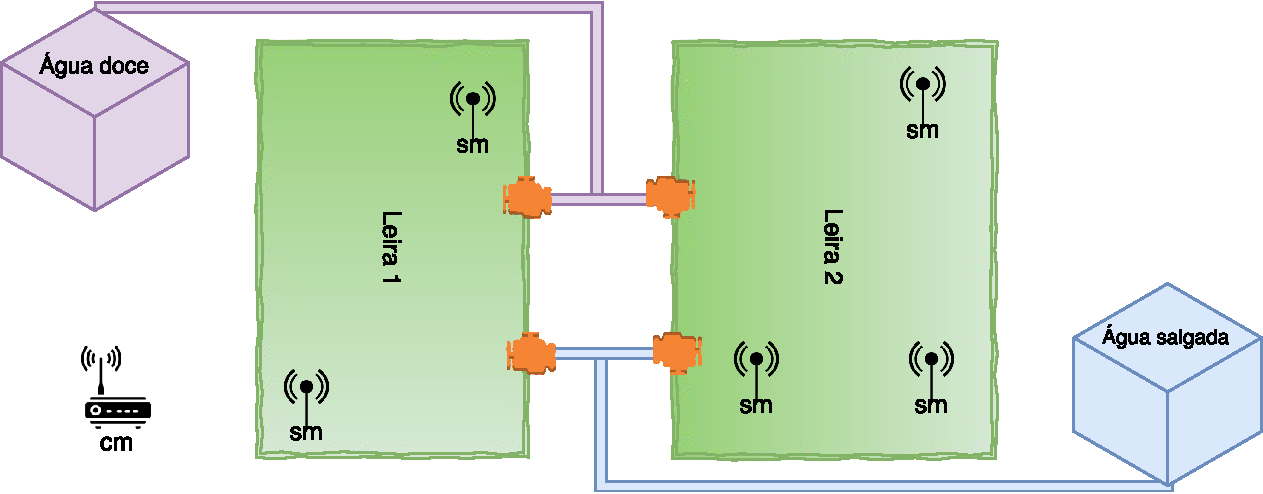
\includegraphics[scale=0.55]{esquemas/leiras-comm-geral.pdf}
	\caption{Ilustração de uma "quinta" onde se produz salicornia}
	\label{leira}
\end{figure}


 
 
Neste contexto, cada grupo de sensores espalhado por cada leira irá comunicar com um módulo central, originando uma topologia de rede em estrela.  Por sua vez, este módulo irá comunicar diretamente com a servidor que possibilitará que os dados sejam tratados e disponíveis para visualização ao cliente. Pressupõe-se portanto que este ultimo módulo tenha necessariamente ligação à rede de modo a conseguir consumir a API REST por HTTP desenvolvida para o efeito. 



\newpage
\section{Componentes}

No contexto desta dissertação é necessário reter dois conceitos principais, são eles: 

\begin{itemize}
	\item \textbf{\textit{\acl{SM}}:} consiste num microcontrolador responsável pela aquisição de dados provenientes dos mais diversos tipos de sensores. Cada \textit{sensor module} terá que utilizar um determinado módulo de comunicação de modo a possibilitar a comunicação com um módulo central. Para além disso, pretende-se que o sensor module possa ter controlo sobre si, ou seja, inteligência própria.
	 
	\item \textbf{\textit{\acl{CM}}:} consiste num microcontrolador responsável pela receção dos dados preveniente dos \textit{sensor modules}. Pretende-se que este módulo envie informações para os sensor modules quando requisitados pelo utilizador. O principal objetivo deste módulo consiste em receber a informação proveniente dos sensor modules e respectivo envio para o servidor em cloud. 
	
	
\end{itemize}


A figura \ref{esquema1}, ilustra a comunicação entre três sensor modules com um controller moduler. Cada um desses sensor modules possui um conjunto especifico de sensores que comunica com controller module através de um determinado modulo de comunicação. Posteriormente, o controller module possui um determinado protocolo de comunicação que permite a utilização da API REST. 


\begin{figure}[h]
	\centering
	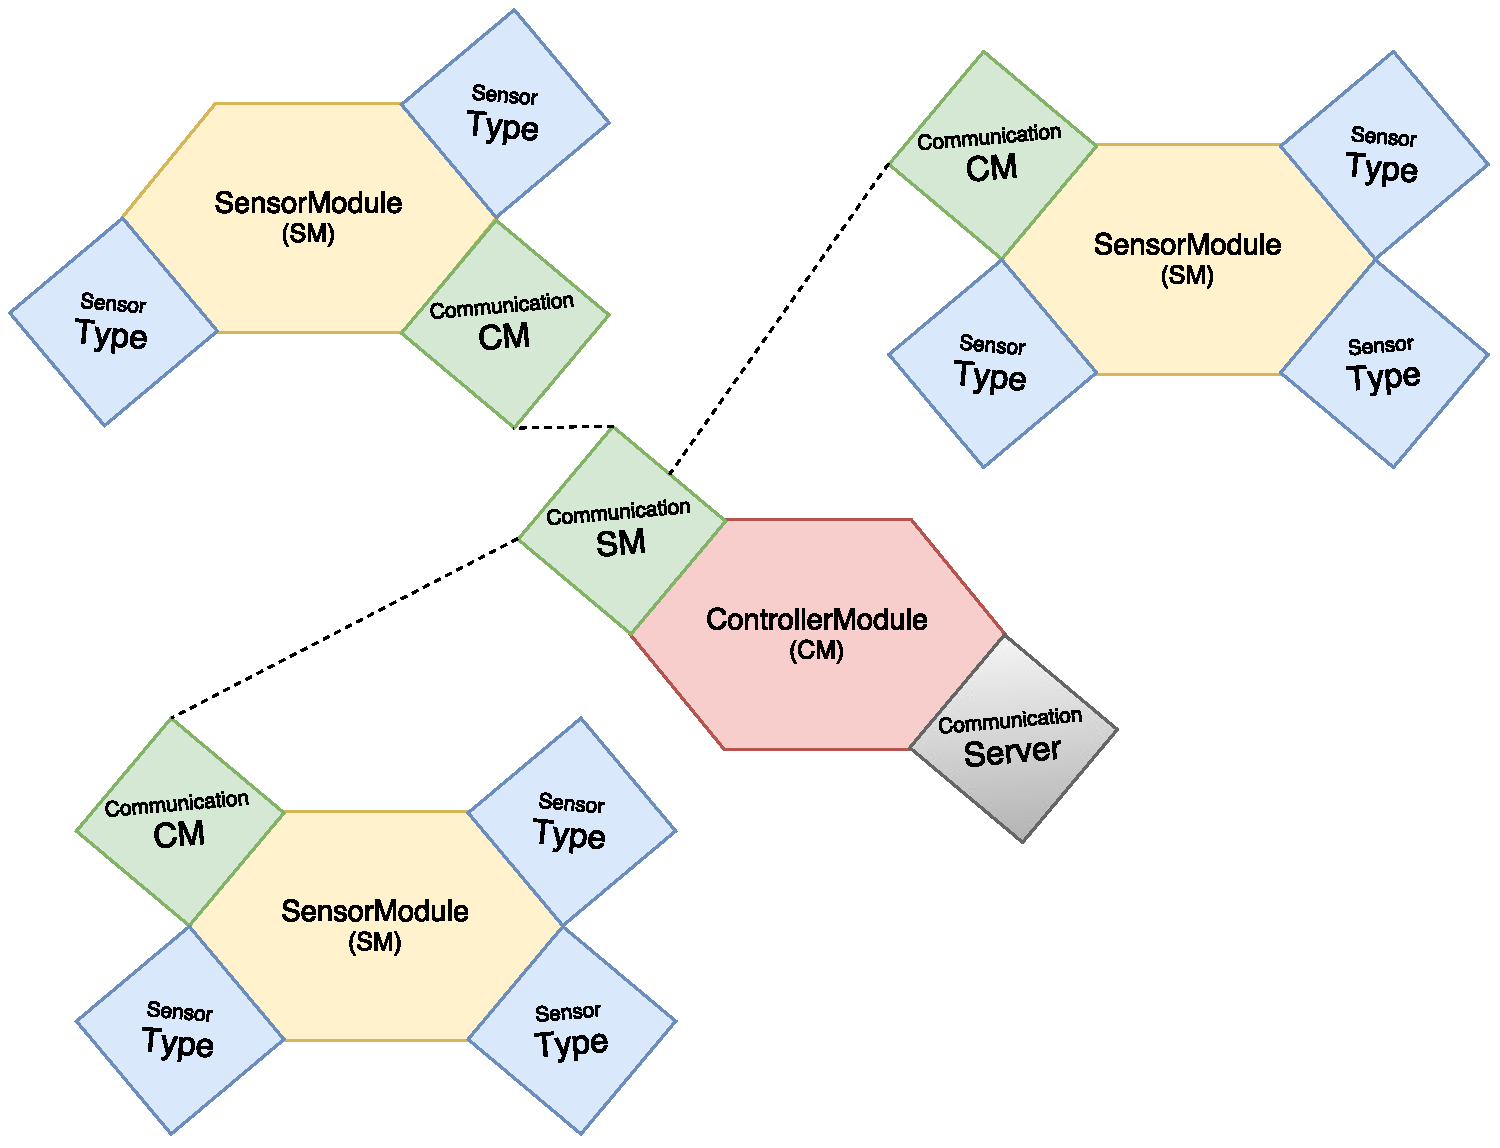
\includegraphics[width=\linewidth]{esquemas/general-electronic-modules.pdf}
	\caption{Pirâmide do conhecimento: modelo DIKW}
	\label{esquema1}
\end{figure}


Seguidamente serão especificados todos os detalhes de cada modulo, uma vez que serão considerados na modulação deste sistema de informação. 

\subsection{Controller Module}

nome
bateria
memoria
comunicacao
localizacao


\subsection{Sensor Module}


nome
tipos de senores 
tempo em que é recebida info 
bateria
localizacao



\newpage

%\section{Design funcional}






\section{Análise de requisitos}

Durante o desenvolvimento um software pressupõe-se que os seus intervenientes sigam determinadas metodologia para o seu programa possa revolucionar a vida de um grupo em especifico ou até mesmo da sociedade. 


O ciclo de vida do desenvolvimento de um software, também conhecido como \ac{SDLC}, é composto genericamente por quatro fase principais: concepção, projeto, criação e a implementação. Antes do \ac{SDLC}, o processo de desenvolvimento do software foi tomado como atividade informal sem regras e padrões formais. Isso poderá levar a vários problemas, tais como o atraso no desenvolvimento, aumento de custos e baixa qualidade do software criado. 

O ciclo de vida do desenvolvimento de um software dá o padrão necessário e as etapas para o desenvolvimento de um software com qualidade. Existem enumeros modelos e visões para o ciclo de vida de desenvolvimento, o que a seguir descrevo foi considerado por Munish Kaur \cite{Saini2014}. A figura \ref{sdlcartic} mostra as várias etapas que compõe este modelos e que seguidamente são descritas. 


\begin{figure}[!htb]
	\centering
	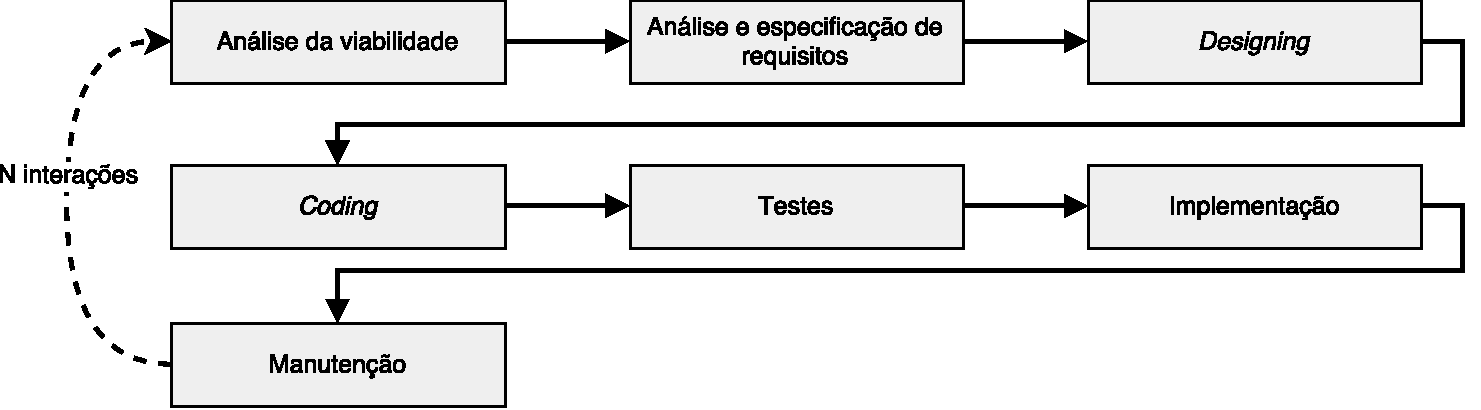
\includegraphics[scale=0.6]{esquemas/desenvolvimentoSW.pdf}
	\caption[Fase de desenvolvimento de um software ]{Fase de desenvolvimento de um software (Adaptado de \cite{Saini2014})}
	\label{sdlcartic}
\end{figure}




\begin{itemize}
	\item Análise de Viabilidade: Nesta fase, a viabilidade do projeto está sendo avaliada em termos de dados de entrada, dados de saída, processamento necessário para transformar a entrada para a produção necessária, análise de custo e planejamento do projeto. Ele também inclui a viabilidade técnica em termos de software, hardware e pessoas qualificadas. No final do estudo de viabilidade é gerado o relatório de viabilidade.
	
	\item \textbf{Analise e especificação de requisitos}: nesta fase são recolhidos e analisados os requisitos necessário para a elaboração do \textit{software}. Pretende-se que no final desta fase sejam conhecidos os vários requisitos do software e seja também criado um documento que os especifique. 
	
	\item  \textbf{\textit{Designing}}: consiste na tradução dos requisitos especificado na fase anterior para a estrutura lógica.Pretende-se que seja elaborado um documento de especificação do \textit{design}. 
	
	
	\item  \textbf{\textit{Coding}}: o programação real é elaborada nesta fase. O documento de \textit{design} é traduzido para o código-fonte numa determinada linguagem de forma a que possa ser executado. 
	
	\item \textbf{Testes}: o código-fonte gerado na fase anterior é testado usando vários cenários de testes. São usadas várias técnicas de teste para avaliar a correção e validação do \textit{software}. 
	
	\item  \textbf{Implementação}: o software desenvolvido é implementado para que possa ser disponbilizado ao utilizador para uso real. Pretende-se que o utilizado do sistema possa reportar erros ou problemas quando encontrados. 
	
	\item  \textbf{Manutenção}: o software poderá sofrer alterações que possam solucionar problemas que tenham ocorrido. Esta fase é responsável pela pós-implementação e manutenção do software para o seu bom funcionamento.
	
\end{itemize}




%





%http://www.sersc.org/journals/IJSEIA/vol8_no3_2014/38.pdf




A forma como um software realiza as tarefas para as quais foi desenvolvido determina a eficiência de execução do mesmo. 
% http://wer.inf.puc-rio.br/WERpapers/pdf_counter.lua?wer=WER03&file_name=leandro_audy.pdf 





O levantamento de requisitos é umas das partes mais importantes do processo que resultará no desenvolvimento de um determinado sistema. Entender aquilo que o cliente deseja ou o que o cliente acredita que precisa e as regras do negócio ou processos do negócio. Isso é o o fator determinante que move essa importante função que faz parte da Engenharia de Software(Engenharia de requisitos). 

% http://www.klebermota.eti.br/wp-content/aluno_leandro_cicero_levantamento_de_requisitos.pdf 



\subsection{Requisitos funcionais}


Os requisitos funcionais descrevem os critérios que devem ser usados para avaliar as funções especificas ou os comportamentos de um determinado sistema. Seguidamente são apresentados os requisitos funcionais propostos pelo cliente no contexto deste projeto para as duas plataformas disponíveis: web (dashboard) e mobile. 


\textbf{Aplicação mobile (dashboard)}


\begin{itemize}
	\item A interface do sistema deve permitir que o utilizador, seja ele qual for, entre ou faça \textit{login} no sistema. 
	
	\item A interface do sistema deve permitir que o utilizador, seja ele qual for, saia ou faça \textit{logout} no sistema.
	
	\item O dashboard deverá permitir que qualquer utilizador possa recuperar a sua chave de acesso ao sistema.
	
	\item O sistema deve permitir que qualquer utilizador se possa registar no sistema, embora tenha que estar obrigatoriamente associado a uma empresa.
	
	\item O utilizador comum só terá acesso à sua área reserva após a validação por parte da empresa.   
	
	\item O dashboard deverá permitir ao administrador a adição de novas empresas e a gestão de todos os utilizadores. 
	
	\item O sistema deve permitir que qualquer utilizador possa adicionar, editar ou remover: 
	\begin{itemize}
		\item Tipos de sensores
		
		\item Tipos de comunicação
		
		\item Controller modules com as suas caracteristicas
		
		\item Tipo de comunicação a um controller modules que permite a comunicação como servidor 
		
		\item Sensor modules a um determinado controller modules e as suas características 
		
		\item Um ou vários tipos de comunicação de um Sensor moduel
		
		\item Um ou vários sensores a um sensor module em que cada sensor é de um determinado tipo 
		
	\end{itemize}
	
	\item Visualizar graficamente os dados de cada sensor para um determinado \ac{SM}. 
	
	
	\item Visualizar em modo tabular (dataset) os dados de cada sensor para um determinado \ac{SM}. 
	
	\item Em cada uma das visualizações anteriormente descritas, pretende-se que seja possível uma filtragem por data
	
	
	\item O sistema permitirá a exportação dos dados de um determinado \ac{SM} em formato \ac{CSV}. 
	
	
	\item  Consultar a documentação da API 
	
	\item Consultar o token de autenticação da API 
	
	
	\item Alterar configurações do utilizador 
	
	
	
\end{itemize}


\textbf{Aplicação mobile}



\begin{itemize}
	\item A interface da aplicação mobile deve permitir que o utilizador, seja ele qual for, entre ou faça \textit{login} no sistema. 
	
	\item A interface da aplicação mobile deve permitir que o utilizador, seja ele qual for, saia ou faça \textit{logout} no sistema.
	
	
	\item Visualizar graficamente os dados de cada sensor para um determinado \ac{SM}. 
	
	\item Receber alarmes quando um determinado valor lido está fora do estipulado.
	
	
\end{itemize}



\subsection{Requisitos não funcionais}


Requisitos não funcionais são todos os requisitos da aplicação relacionados com
performance, escalabilidade, segurança, disponibilidade e usabilidade. Estes não são
necessariamente pedidos pelo cliente. 


\begin{itemize}
	\item O sistema deverá executar em qualquer plataforma.
	
	\item O sistema deverá disponibilizar uma API para que possam ser criados novos produtos com base neste 
	
	
\end{itemize}



\newpage
\section{Modelação}
\subsection{Entidades envolventes}




No contexto do sistema descrito existem três entidades distintas que são importantes descrever: 

\begin{itemize}
	
	\item \textbf{General user}: este poderá registar-se e associando-se a uma determinada empresa registada no sistema. Após a validação por parte da empresa, este utilizador poderá aceder à sua área reservada através das dashboard ou aplicação mobile. 
	
	\item \textbf{Companny user}: utilizador que gere todos os general users que se possam associar à sua empresa. Deste modo, este utilizador poderá validar os general users que a si se associam ou eliminá-los caso a permissão não seja desejada.  
	
	\item \textbf{Administrador}: vulgarmente denominado por Admin. Pretende-se que apenas exista uma único administrador. Genericamente este utilizador tem a possibilidade de poder adicionar novas empresas ao sistema i.e. criar novas utilizador com permissões especificas. 
	
\end{itemize}



\newpage

\subsection{Casos de uso}


\begin{figure}[!htb]
	\centering
	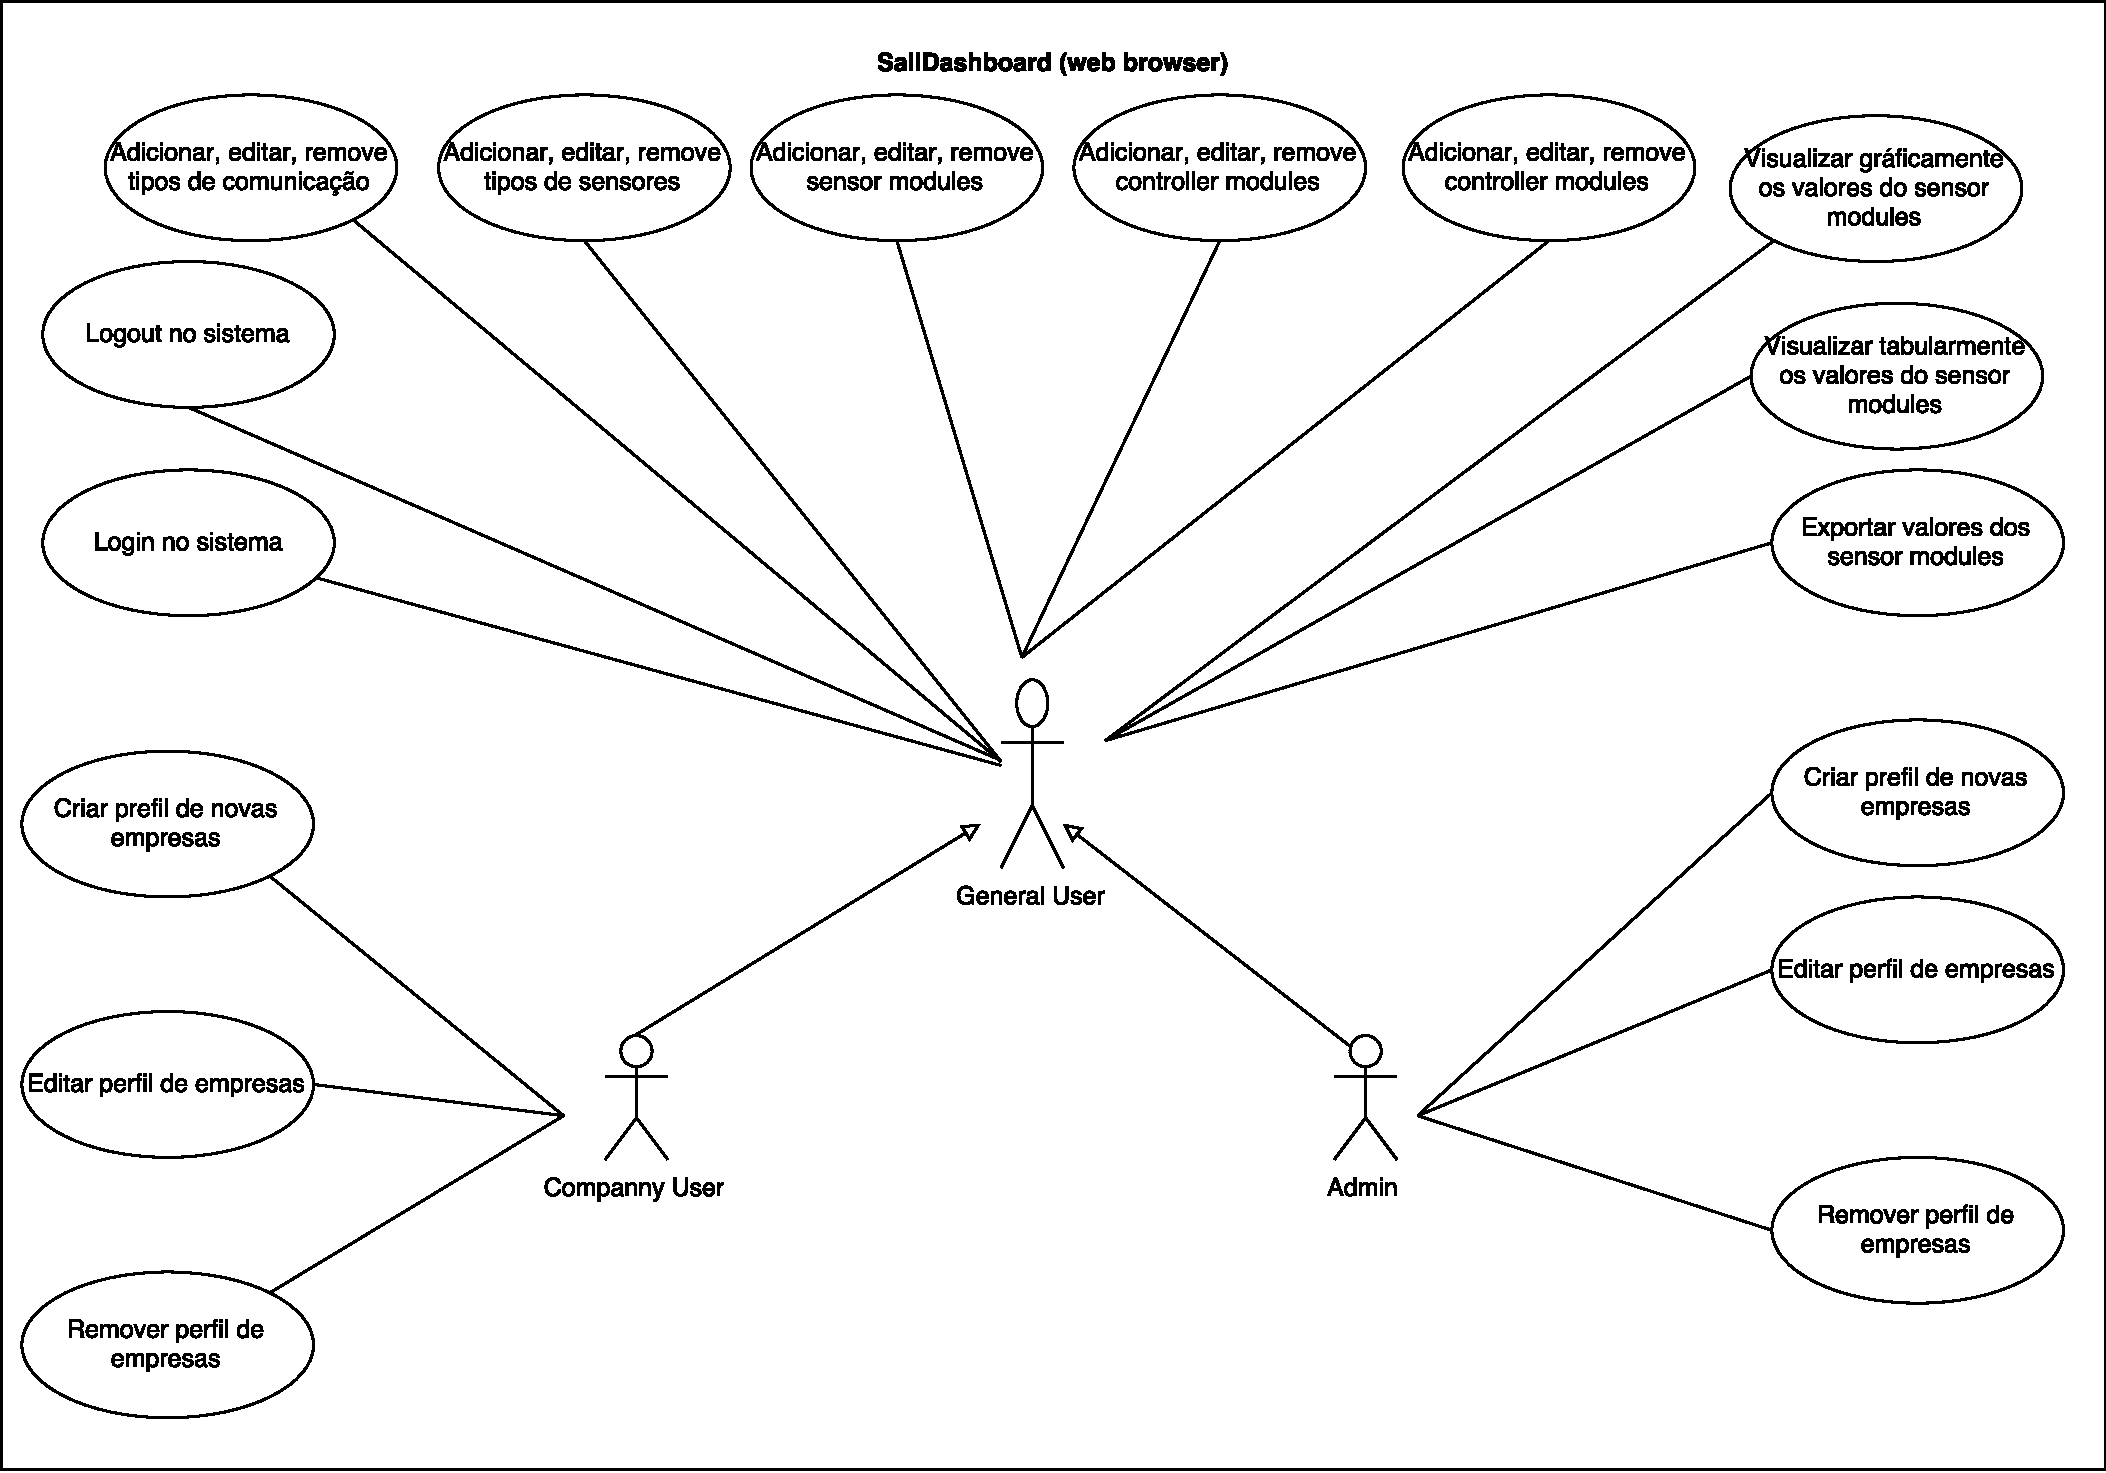
\includegraphics[width=\linewidth]{esquemas/use-case-web.pdf}
	\caption{Pirâmide do conhecimento: modelo DIKW}
	\label{dikw}
\end{figure}


\begin{figure}[!htb]
	\centering
	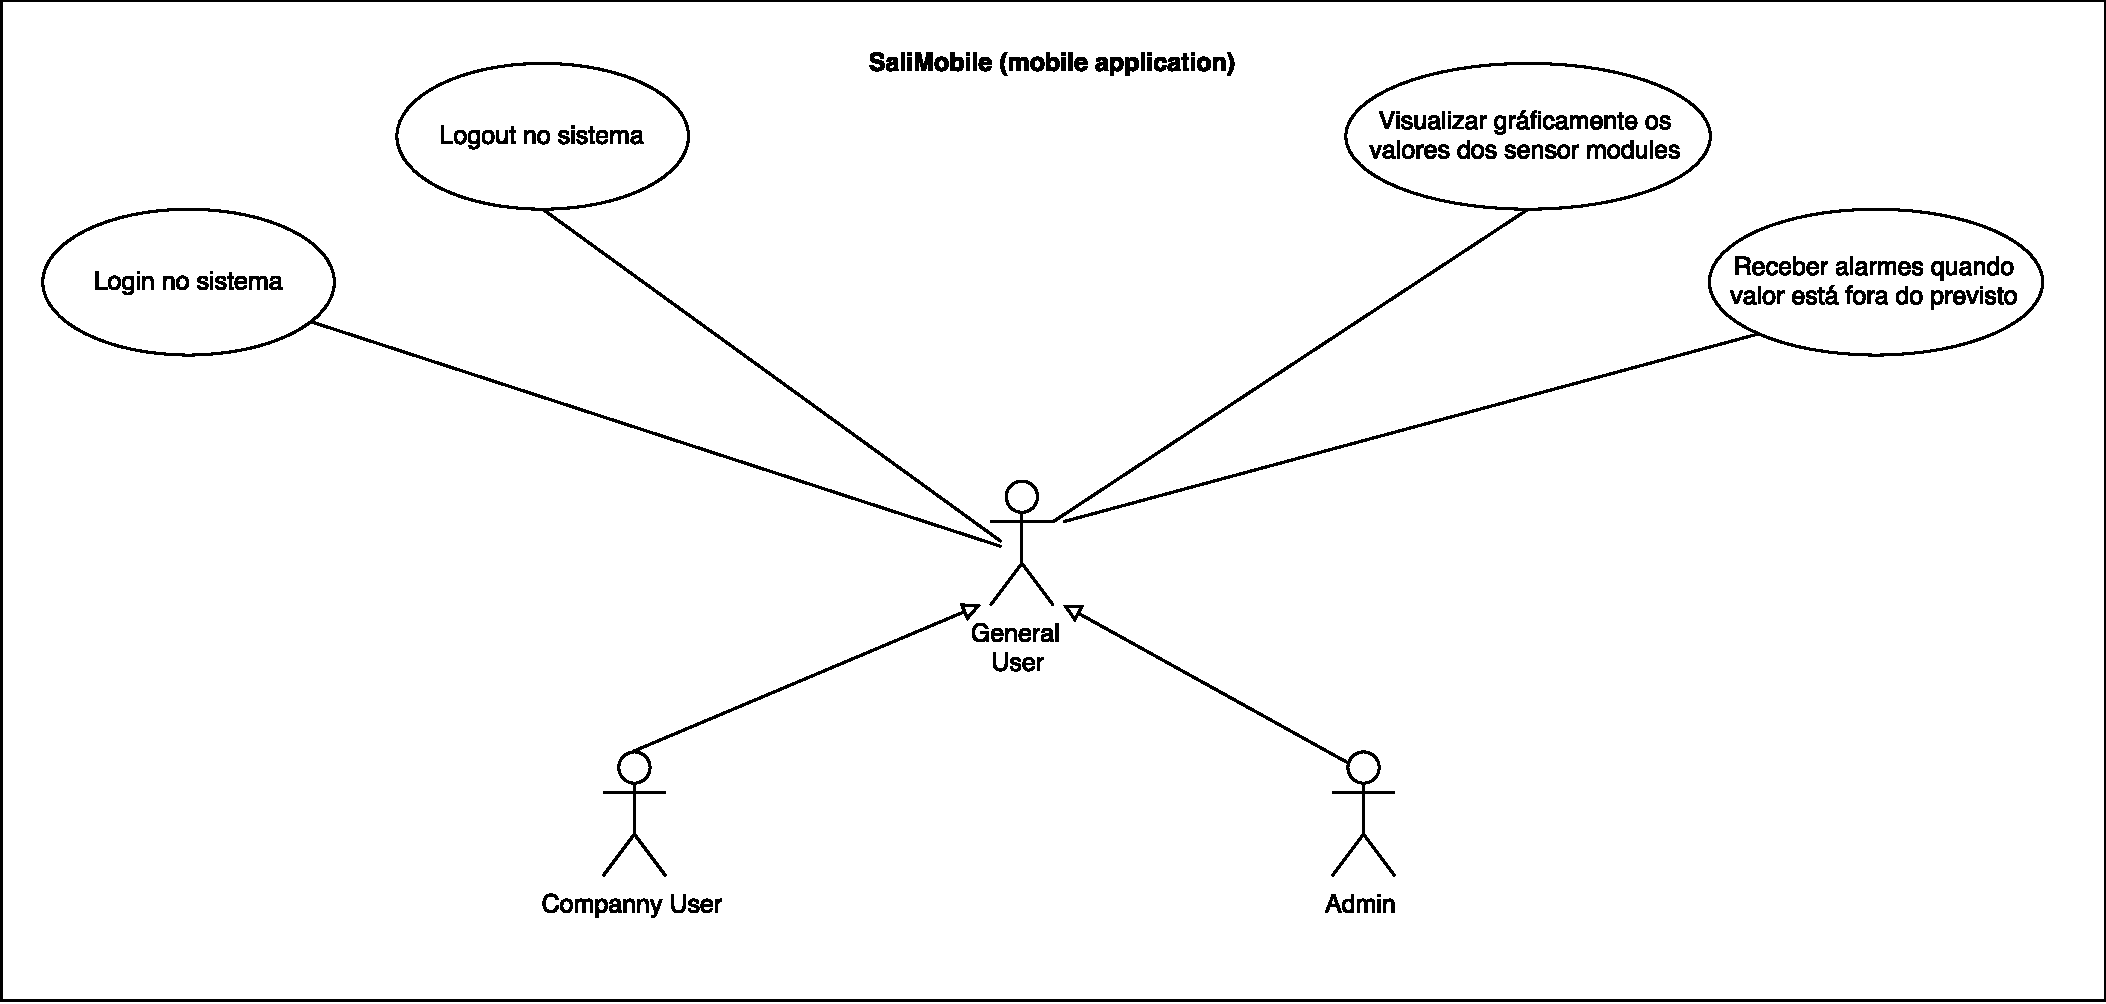
\includegraphics[width=\linewidth]{esquemas/use-case-mobile.pdf}
	\caption{Pirâmide do conhecimento: modelo DIKW}
	\label{dikw}
\end{figure}



\newpage
\subsection{Modelo de dados}


\begin{figure}[!htb]
	\centering
	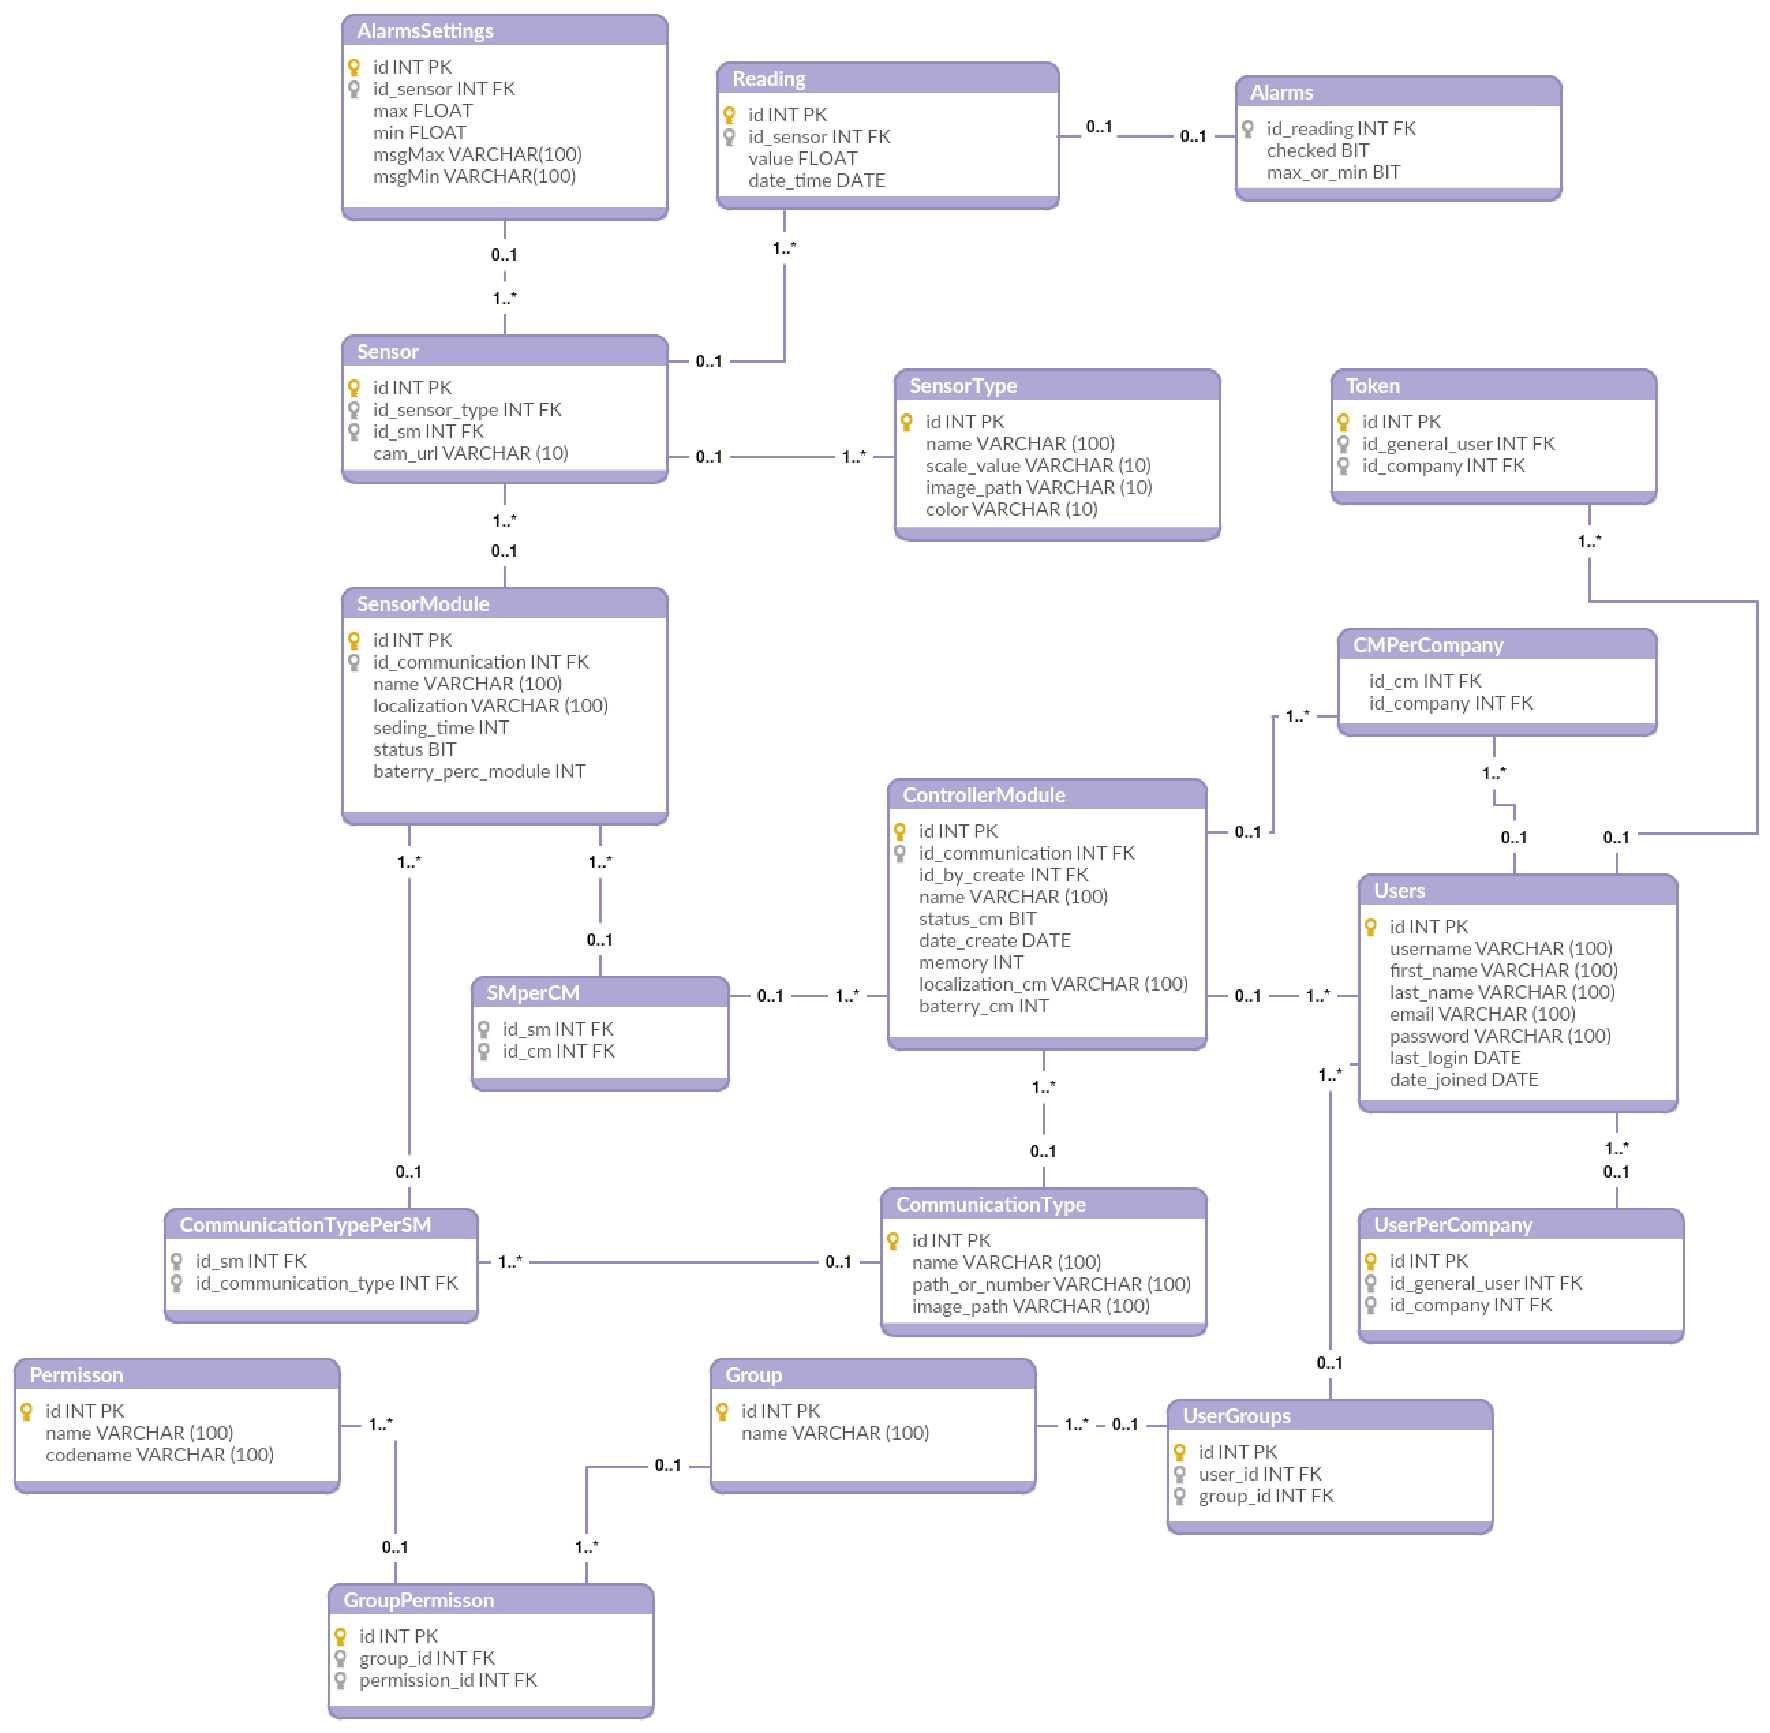
\includegraphics[width=\linewidth]{esquemas/database_tese.pdf}
	\caption{Pirâmide do conhecimento: modelo DIKW}
	\label{db}
\end{figure}


\newpage

\begin{table}[h]
	\centering
	\begin{tabular}{|l|l|l|}
		\hline
		\multicolumn{1}{|c|}{\textbf{Nome}} & \multicolumn{1}{c|}{\textbf{Identificador}} & \multicolumn{1}{c|}{\textbf{Descrição}} \\ \hline
		User & auto-incrementado & dasdas \\ \hline
		ControllerModule&  &  \\ \hline
		SensorModule&  &  \\ \hline
		CommunicationType&  &  \\ \hline
		SensorType&  &  \\ \hline
		Sensor&  &  \\ \hline
		Reading&  &  \\ \hline
		AlarmsSettings&  &  \\ \hline
		Alarms&  &  \\ \hline
	\end{tabular}
	\caption{My caption}
	\label{my-label}
\end{table}









\newpage
\section{Arquitetura lógica}

Normalmente este tipo de arquitetura é composto por: camada de apresentação,
camada de lógica de negócio e camada de acesso a dados.


\begin{figure}[!htb]
	\centering
	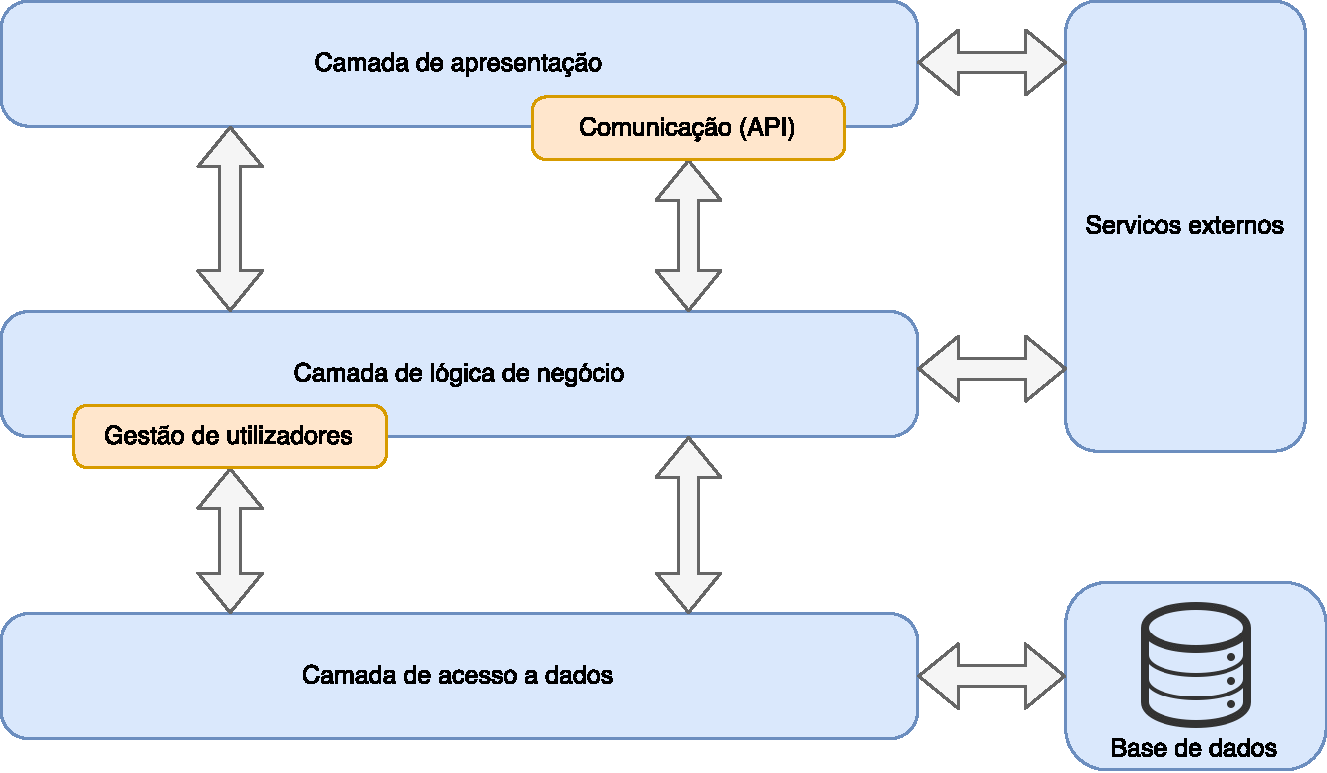
\includegraphics[width=\linewidth]{esquemas/arquitetura-logica.pdf}
	\caption{Arquitetura lógica}
	\label{opencvlogo}
\end{figure}



\subsection{Camada de apresentação}


A camada de apresentação é responsável pela comunicação entre os utilizadores e a aplicação, sendo ela web ou mobile, exibindo informações aos utilizadores, abrangendo uma interface que permite solicitações ao sistema. Esta camada tem uma relação de dependência com a camada de lógica de negócio e tira partido do acesso a serviços de informação externos, que fornecem diversas funcionalidades. 


A interface do utilizador foi desenvolvida em  \ac{HTML} e \ac{CSS}, fazendo uso de jQuery e Javascript.



\begin{itemize}
	\item \ac{HTML} é a linguagem padrão usada para estruturar e apresentar conteúdos na web. Neste caso, foi utilizado HTML5, a quinta versão do \ac{HTML}.
	\item \ac{CSS} é uma linguagem usada para descrever a apresentação de conteúdo escrito em uma marcação Como HTML.
	\item Javascript é a linguagem de programação para páginas da web.
	\item \textbf{JQuery}: JQuery é uma biblioteca Javascript que simplifica a programação Javascript
\end{itemize}









\subsection{Camada de lógica de negócio}



\subsection{Camada de acesso a dados}


Nesta camada deverão estar presentes as funcionalidades de criação, edição, remoção ou simples de visualização dos dados, sendo responsável pelas operações
de persistência e consulta de dados solicitadas pela camada de lógica de negócio.



\section{Arquitetura física}


\subsection{Sistema de informação}



\subsubsection{\ac{API}}

Os métodos da API permitem executar as funções REST. Assim, torna-se fundamental perceber estes métodos para ter um melhor conhecimento do funcionamento do sistema. Como tal, de seguida, são descritos os métodos mais importantes que dão suporte a cada uma das funções REST.

\begin{itemize}
	\item \textbf{GET}: 
	\item \textbf{POST}: 
	\item \textbf{DELETE}: 
\end{itemize}





\begin{table}[h]
	\centering
	\begin{tabular}{|l|l|l|}
		\hline
		\multicolumn{1}{|c|}{\textbf{End point}} & \multicolumn{1}{c|}{\textbf{Tipo}} & \multicolumn{1}{c|}{\textbf{Descrição}} \\ \hline
		User & auto-incrementado & dasdas \\ \hline
		ControllerModule&  &  \\ \hline
		SensorModule&  &  \\ \hline
		CommunicationType&  &  \\ \hline
		SensorType&  &  \\ \hline
		Sensor&  &  \\ \hline
		Reading&  &  \\ \hline
		AlarmsSettings&  &  \\ \hline
		Alarms&  &  \\ \hline
	\end{tabular}
	\caption{My caption}
	\label{my-label}
\end{table}

Autenticação

Documentação automática



%\section{Documentação automática}

%\subsection{Documentação API}

utilizado swagger; apenas permite acesso a quem está logado... incorporar layout do swagger com o do salidashboard




\newpage




\subsection{Aplicação web}


\subsection{Aplicação mobile}




\newpage
\subsection{Simulação em hardware}

Após a desenvolvimento da API descrita no capitulo anterior, pretendeu-se simular o sistema num contexto real. Para tal, planeou-se encontrar hardware que encaixasse no contexto deste projeto. Foram utilizados dois micro-controladores e alguns sensores. Neste capitulo será descrito cada um deles e o processo de desenvolvimento da respetiva simulação.  

\newpage

\subsubsection{Sensores utilizados}

Nesta secção serão apresentados os sensores utilizados na simulação e as suas principais características. Todos os sensores foram escolhidos tendo em conta o seu enquadramento no projeto e a sua disponibilidade no laboratório. Todos os sensores que se apresentam encontram-se ligados a um Arduino nano. \\


\textbf{Temperatura}


Como sensor de temperatura foi utilizado um termístor do tipo \ac{NTC}. Como vimo anteriormente, um termístor é um semicondutor sensível à temperatura i.e. cujo o coeficiente de variação da resistência com a temperatura é negativa, ou seja, quando a temperatura sobe então consequentemente a resistência diminui. 

Na figura \ref{esquema-temp} encontra-se o esquema de ligação deste componente e na tabela \ref{table-temp} as propriedades principais. 

\begin{figure}[h]
	\centering
	\begin{minipage}[b]{0.4\textwidth}
		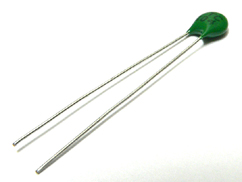
\includegraphics[width=\textwidth]{img/hardware/temperatura.jpg}
		\caption{TTC 104 NTC}
	\end{minipage}
	\hfill
	\begin{minipage}[b]{0.4\textwidth}
		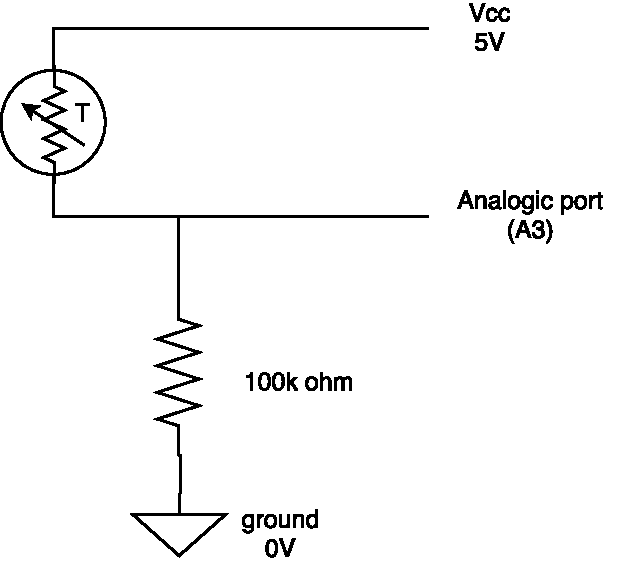
\includegraphics[width=\textwidth]{img/hardware/temp-esquema.pdf}
		\caption{Esquema eletrotécnico da ligação do sensor de temperatura}
		\label{esquema-temp}
	\end{minipage}
\end{figure}



\begin{table}[h]
	\centering
	
	\begin{tabular}{|
			>{\columncolor[HTML]{C0C0C0}}l |l|} \hline
		Dimensão & 5mm \\ \hline
		Resistência & 100K $\Omega$  \\ \hline
		Valor máximo & +125C \\ \hline
		Valor mínimo & -30C \\ \hline
		Nível de confiança & + - 10\% \\ \hline
		Preço & 0.35 \euro/unidade \\ \hline
	\end{tabular}
	\caption[Características do sensor TTC 104]{Características do sensor TTC 104 \cite{temp-dta}}
	\label{table-temp}
\end{table}


\newpage
\textbf{Luminosidade}

Para simular a luminosidade incidente foi utilizado um sensor do tipo foto-resistência. Este sensor, também conhecido como \ac{LDR}, não é mais do que uma resistência variável cujo o seu valor varia conforme a intensidade da luz que incide sobre ele i.e. à medida que a intensidade da luz aumenta, a sua resistência diminui. Este sensor tem múltiplas aplicações, entre as quais se destaca a monitorização solar, indicador da posição do sol (up/down), alarmes anti-roubo, alarme para abertura/fecho de portas entre outras. 

Como vimos na secção X do capitulo do Estado de Arte é um sensor de baixo custo e bastante fácil de utilização. Na figura \ref{lum-esquema} encontra-se o esquema de ligação do componente e na tabela \ref{lum-cara} são apresentadas as principais características do sensor utilizado. 







\begin{figure}[h]
	\centering
	\begin{minipage}[b]{0.4\textwidth}
		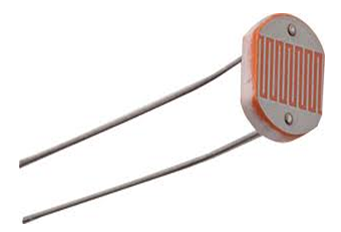
\includegraphics[width=\textwidth]{img/hardware/luminosidade.png}
		\caption{Sensor foto-resistência GL5528}
	\end{minipage}
	\hfill
	\begin{minipage}[b]{0.4\textwidth}
		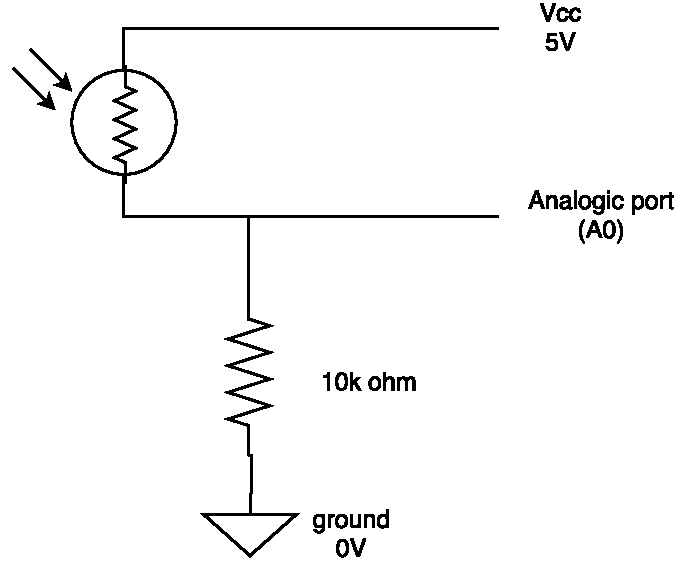
\includegraphics[width=\textwidth]{img/hardware/lumi_esquema.pdf}
		\caption{Esquema eletrotécnico da ligação do sensor de luminosidade}
		\label{lum-esquema}
	\end{minipage}
\end{figure}











\begin{table}[h]
	\centering
	
	\begin{tabular}{|
			>{\columncolor[HTML]{C0C0C0}}l |l|} \hline
		Diâmetro & 5mm \\ \hline
		Tensão máxima & 150VDC \\ \hline
		Potência máxima & 100mW \\ \hline
		Tensão de operação & -30 C a 70 C \\ \hline
		Espectro &540nm \\ \hline
		Comprimento com terminais & 32mm \\ \hline
		Resistência no escuro &1 M (Lux 0) \\ \hline
		Resistência na luz &10-20 Komega (Lux 10) \\ \hline
		Material & Carbono \\ \hline
		Preço & 0.22 \euro/unidade \\ \hline
	\end{tabular}
	\caption[Características do sensor GL5528]{Características do sensor GL5528 \cite{lum-data}}
	\label{lum-cara}
\end{table}


\newpage

\textbf{Sensor de nível líquido}

Este sensor não é mais do que um interruptor que é ativo sempre que um determinado líquido ultrapassa o mesmo. Sempre que algum líquido atingir o pedaço de plástico este irá subir ativando assim o circuito. 
Na figura \ref{esquem-liquido} encontra-se o esquema da ligação deste sensor.




\begin{figure}[h]
	\centering
	\begin{minipage}[b]{0.4\textwidth}
		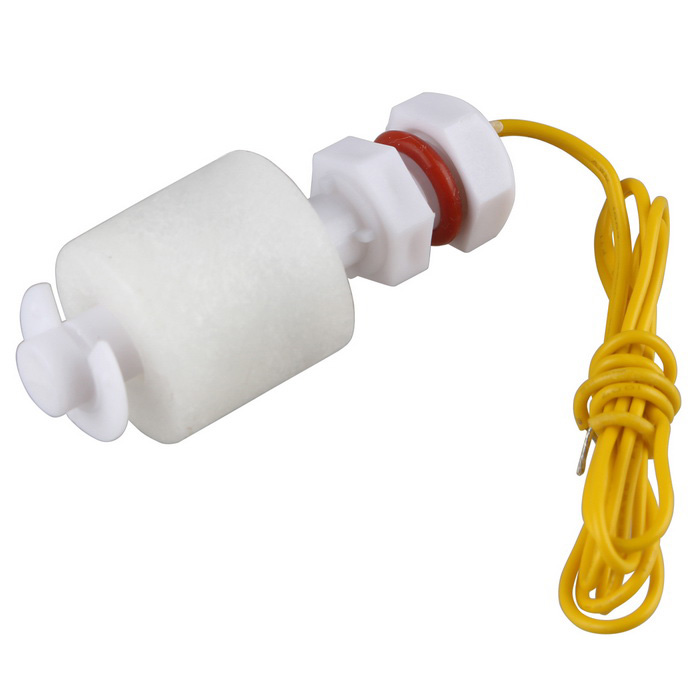
\includegraphics[width=\textwidth]{img/hardware/liquido.JPG}
		\caption{\textit{Water Level Switch Liquid Level Sensor Plastic Ball Float}}
	\end{minipage}
	\hfill
	\begin{minipage}[b]{0.4\textwidth}
		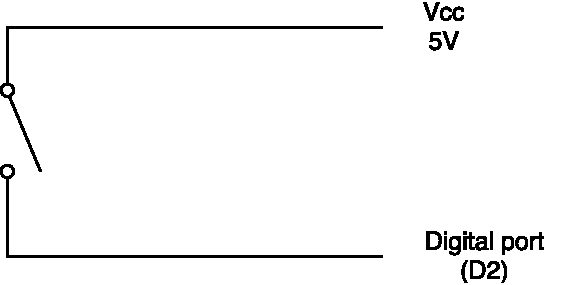
\includegraphics[width=\textwidth]{img/hardware/sw_esquema.pdf}
		\caption{Esquema eletrotécnico da ligação do sensor de nível líquido}
		\label{esquem-liquido}
	\end{minipage}
\end{figure}



\textbf{Simulador de válvula para transferências de águas}

Para a simulação de uma válvula que permitirá as transferência de água doce e salgada foi utilizado um simples \textit{led}. Este possibilita facilmente identificar através da ativação do \textit{led} se a válvula se encontra ativa ou não. 


\begin{figure}[h]
	\centering
	\begin{minipage}[b]{0.4\textwidth}
		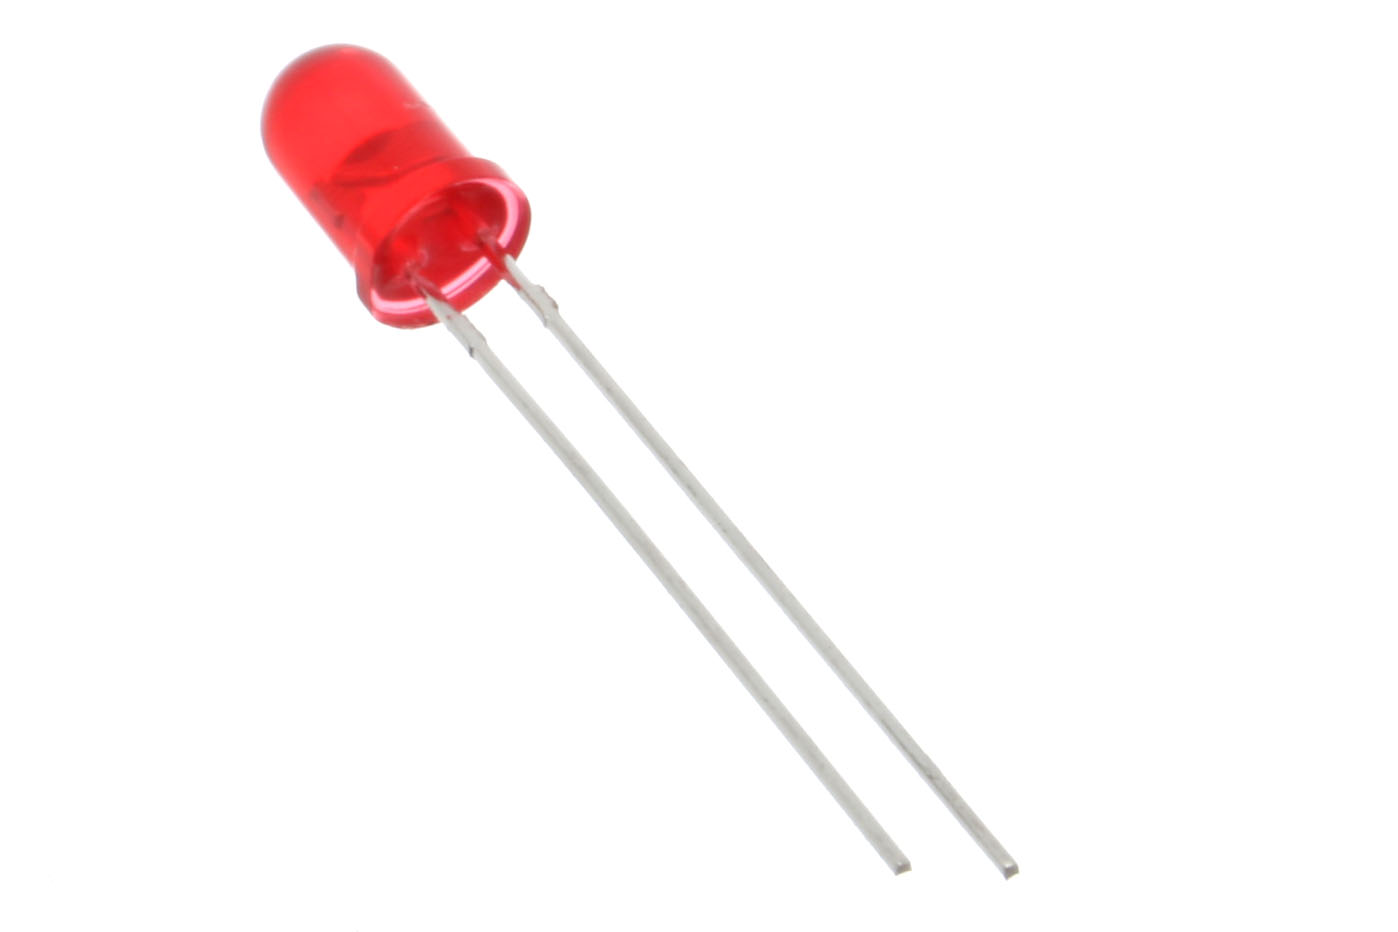
\includegraphics[width=\textwidth]{img/hardware/led.jpg}
		\caption{Led simples.}
	\end{minipage}
	\hfill
	\begin{minipage}[b]{0.4\textwidth}
		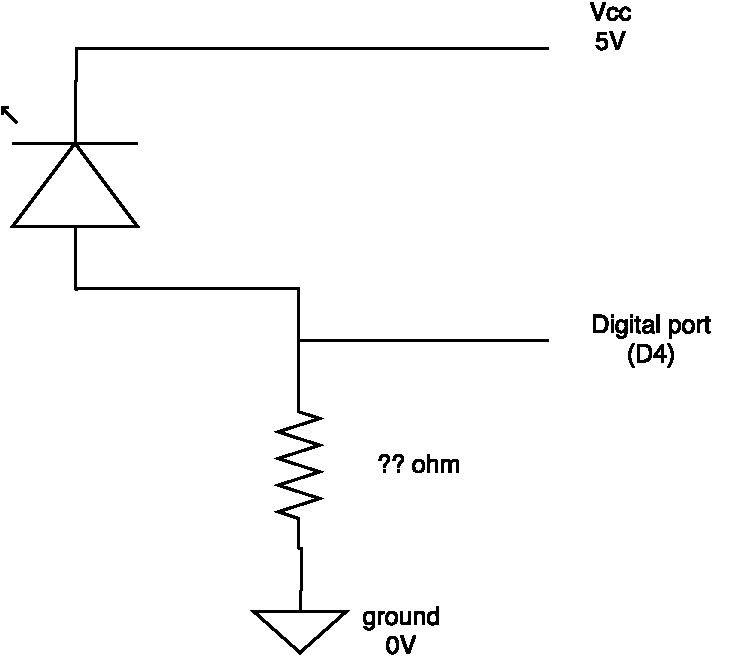
\includegraphics[width=\textwidth]{img/hardware/led_esquema.pdf}
		\caption{Esquema eletrotécnico da ligação do led}
	\end{minipage}
\end{figure}




\newpage
\subsubsection{Comunicação}

Nesta secção, será apresentado o tipo de comunicação para este cenário de simulação. Pretendeu-se que cada um dos módulo ficassem isolados entre si, o que implicou o estudo e respetiva escolha de algumas tecnologias de comunicações sem fio. Neste caso, foram escolhidas as seguintes: 

\begin{itemize}
	\item \textbf{Bluetooth}: utilizado para a comunicação entre o Arduino (\ac{SM}) e o Raspberry Pi 3 (\ac{CM}). No Arduino foi utilizado um módulo Bluetooth HC-06 e no Raspberry Pi 3 foi utilizado o seu próprio módulo interno. 
	\item \textbf{Wifi}: utilizado para a comunicação entre o Raspberry Pi 3 (\ac{CM}) e o servidor. 
\end{itemize}


O esquema da figura \ref{esquemcomm} pretende esquematizar os tipos de comunicação envolvidos nesta simulação para cada um dos componentes. 

\begin{figure}[!htb]
	\centering
	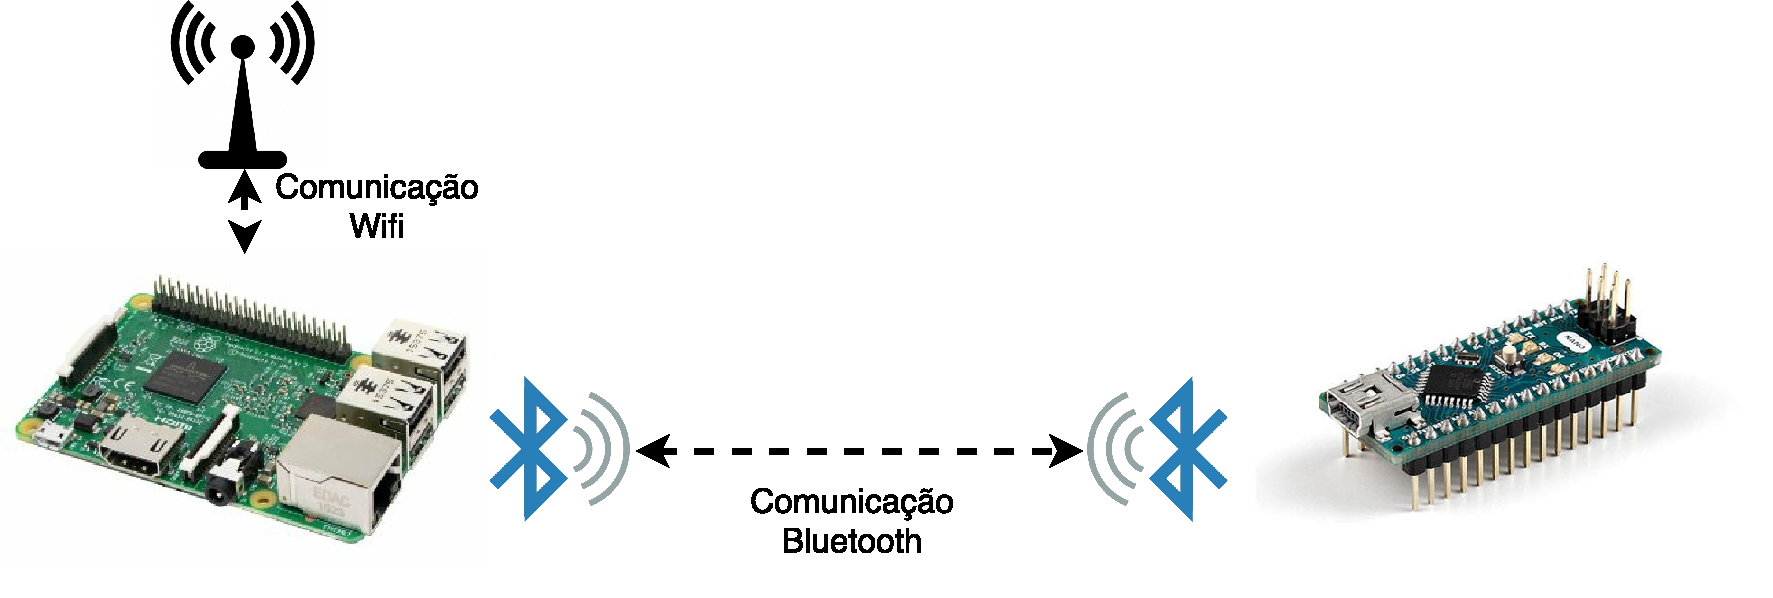
\includegraphics[width=\linewidth]{img/comm-blue/HW-geral.pdf}
	\caption{Arquitetura lógica}
	\label{esquemcomm}
\end{figure}




Módulo bluetooth HC-06



Este módulo bluetooth HC-05 oferece uma forma fácil e barata de comunicação com seu projeto Arduino. Diferente do modelo HC-06, suporta tanto o modo mestre como escravo, além de ter uma fácil configuração.

Em sua placa existe um regulador de tensão e você poderá alimentar com 3.3 a 5v, bem como um LED que indica se o módulo está pareado com outro dispositivo. Possui alcance de até 10m.

é mais uma forma simples e barata de enviar e receber informações remotamente.


\newpage
\begin{figure}[h]
	\centering
	\begin{minipage}[b]{0.4\textwidth}
		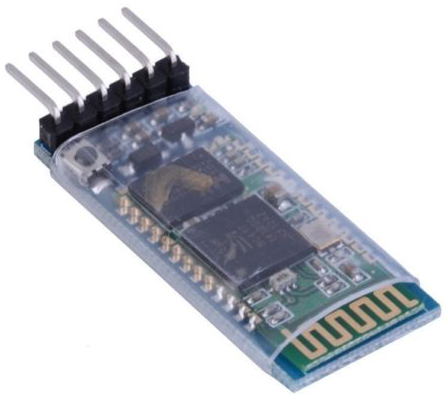
\includegraphics[width=\textwidth]{img/hardware/bluetooth_zs-040.png}
		\caption{Flower one.}
	\end{minipage}
	\hfill
	\begin{minipage}[b]{0.4\textwidth}
		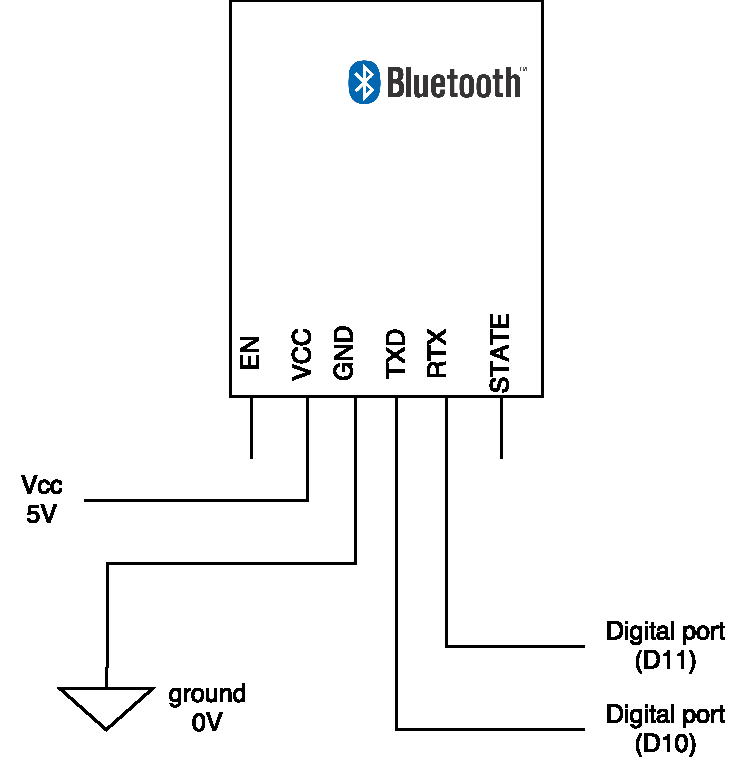
\includegraphics[width=\textwidth]{img/comm-blue/electronic-sensors.pdf}
		\caption{Esquema eletrotécnico da ligação do módulo bluetooth}
	\end{minipage}
\end{figure}



\begin{table}[h]
	\centering
	
	\begin{tabular}{|
			>{\columncolor[HTML]{C0C0C0}}l |l|} \hline
		Diâmetro & 5mm \\ \hline
		
		Protocolo Bluetooth& v2.0+EDR \\ \hline 
		Frequência& 2,4GHz Banda ISM \\ \hline
		Segurança& Autentificação e Encriptação \\ \hline
		Tensão& 3,3v (2,7-4.2v) \\ \hline
		Alcance& 10m \\ \hline
		Dimensões& 26,9 x 13 x 2,2mm \\ \hline
		Peso& 9,6g \\ \hline
		Preço&32\euro /unidade  \\ \hline
	\end{tabular}
	\caption[Características do sensor GL5528]{Características do sensor GL5528 \cite{lum-data}}
	\label{lum-cara}
\end{table}



%http://www.instructables.com/id/Modifying-the-AT-Codes-on-a-HC-05-With-the-Code-ZS/


%http://www.arduinoecia.com.br/2013/03/modulo-bluetooth-jy-mcu-configuracao.html








%%%%%%%%%%%%%%%%%%%%%%%%%%%%%%%%%%%%%%%%%%%%%%%%%%%%%%%%%%

\newpage
\section{Diagrama de componentes}







\newpage








\section{Considerações finais}